
\chapter{Frequency of subject focus-marking strategies}\label{sec:3}
\section{Introduction}
In \chapref{sec:2}, I provided an overview of the different focus-marking strategies discussed so far in the literature for both Spanish and French. The comparison between formal and functional approaches to subject focus has revealed that the theoretical assumptions proposed so far  are only partly corroborated by empirical evidence, and that a more in-depth comparative investigation is needed.

Recent experimental studies have pointed out important variation in the realization of subject focus. Unlike theoretical studies, data-based research has shown that there is more than one means to mark subject focus, and that factors such as diatopic differences \parencite{jimenez2015focus}, register \parencite{destruel2016focus}, argument structure of the verb \parencite{gabriel2007fokus} or the information status of the subject referent \parencite{Karssenberg+2018} might have a considerable impact on the choice of focus-marking strategies.

As has often been pointed out in previous chapters, these contributions, while valuable, present some limitations. First, elicitation tasks, reading tasks, or acceptability judgements have the advantage of offering highly controlled settings and conditions, thereby increasing the comparability of results. However, these same methods reduce speakers' freedom and spontaneity of expression by prompting participants to produce full sentences in response to a visual or auditory stimulus. Consequently, structures such as various types of ellipses, fragments, or reduced clefts are often treated as ``noise” and hence excluded from analysis. Nevertheless, these structures are quite frequent in spontaneous speech, and any exhaustive investigation of subject focus, or focus in general, needs to account for them as well.

Secondly, it is not yet clear whether different focus types (e.g., information focus vs. contrastive/corrective focus) map onto specific syntactic structures, or whether such a mapping can be observed at all. In other words, is there a one-to-one correspondence between contrast vs. information focus and a specific construction (as the Cartographic Approach \textcite{rizzi1997fine} predicts), or are constructions under-specified with respect to their information-structural function? 
The corpus study reported in this chapter captures any structure produced by participants, including not only sentences that exhibit a clear focus-background partition, such as French subject clefts or Spanish postverbal subjects, but also syntactic structures where only the focused constituent is uttered while the background material is elided (e.g., fragments, reduced clefts). The study aims, on the one hand, to investigate the ways in which focused subjects can be expressed in the two languages (along with their respective frequencies) and, on the other hand, to identify possible correlations between focus types and specific syntactic structures.

Thus, the first research question has an exploratory nature. The sentences expressing subject focus are extracted and annotated according to their type. Here, ``type” refers to the syntactic structure under which the pragmatic function is encoded. At this stage, I do not formulate any specific hypothesis or prediction about the possible strategies that speakers might use to convey focus on the subject in the two languages. Rather, the study explores all variants that might compete for the same information-structural function by adopting a Labovian variationist approach \parencite{labov1972sociolinguistic}. Additionally, it investigates whether any correlation can be observed between different focus types (information vs. contrast) and specific answering strategies. As will be shown, both Spanish and French speakers have at their disposal more than one option to encode subject focus, even though some strategies are more frequent than others. The French sub-corpus, for instance, exhibits an elevated number of different cleft formats, while postverbal subjects seem to be the preferred strategy in the Spanish dataset. Interestingly, a high number of elliptical structures can be observed in both sub-corpora. However, the distribution of these answer types varies considerably between the two languages.

This chapter is organized as follows: In \sectref{sub:4.2}, I present the corpus used to conduct the present analysis. \sectref{sub:4.3} and \sectref{sub:4.4} discuss the criteria adopted for the extraction and annotation of the sentences. \sectref{sub:4.5} presents the findings of the Spanish corpus, while \sectref{sub:4.6} reports the results of the French corpus. Finally, \sectref{sub:4.7} and \sectref{sub:4.8} provide a comparative discussion for both languages and a summary of the chapter. 


\section{\textit{Sgs}corpus: General description} \label{sub:4.2}

The data used for the present study is part of the multilingual database \textit{sgs} (speech production -- grammaticality judgments -- social data; \cite{adli2011gradient}). The corpus contains spoken data in four different languages (French, Spanish, Persian and Catalan). It also includes transcription and tree-annotation of spoken language (including primary acoustic data), gradient acceptability judgments, and social structural information. The data was collected in the years 2004, 2005 and 2007. 

The sample of speakers consists of mostly young or middle-aged adults. Each person was first recorded, then asked to participate in a gradient acceptability judgment test, and finally filled out an extensive social questionnaire. 

The Spanish sub-corpus contains data from the Spanish variety spoken in Catalonia which was collected in Barcelona, while the French data was collected in Paris. The empirical design was held constant between field sessions. Each linguistic production of the speaker is transcribed. This transcription facilitates  readability, tree-annotation and the application of the query tools. Being based on spontaneous speech, the \textit{sgs} also contains elements such as hesitation markers, false starts, interjections, and repetitions. 

The French part of \textit{sgs} consists of 102 recorded interviews which contain 44,231 main lines, 51\% of which were produced by 101 interviewees and 49\% by the interviewers. Interviews were carried out in the summer of 2005 with French native speakers between the ages of 19 and 49 (mean age: 29). The sample is composed of 56\% women and 44\% men. 
With regard to the Spanish sub-corpus, the sample consists of 54 recorded interviews containing 10778 (52.7\%) utterances produced by the interviewees and 9662 (47.3\%) by other participants (interviewers or investigator). The sample of participants consists of 54 native speakers of the Spanish variety of Catalonia. 60\% of the sample are women while the other 40\% are men. Participants had completed at least compulsory education, and were between 17 and 48 years old (mean: 28 years). 
The present corpus study considers both the tokens produced by the interviewers and the ones produced by the interviewees.

Importantly, both the Spanish and the French corpus were collected using the same methodological protocol: a game task was developed, where  subjects were instructed to investigate a fictive murder case. This procedure allows participants to choose which aspects of the case they want to talk about. A properly chosen fictive scenario brings subjects into the situation of asking the interviewer questions, while leaving them the freedom to choose the topics. In the scenario, the subject played the part of a police investigator, and the experimenter the doorman of the victim’s building. To maintain spontaneity and authenticity, subjects were instructed to be themselves and not to imitate, for example, some commonly known literary figure.

This game task has the methodological advantage of eliciting a considerable number of question/answer pairs, which, as is well known, facilitates the investigation of focus or, more generally, of different IS-functions. Moreover, the fact that the game task was kept constant for the two languages guarantees optimal conditions for comparability. 

Despite the high comparability and the naturalness of the speech type, the corpus presents some methodological limitations as well. Being in semi-directed interviews, speakers remain aware of the fact that the setting in which they have to interact is somewhat artificial and, most importantly, that they are being observed for linguistic purposes. As has often been pointed out in sociolinguistics, this prevents a fully-natural speech production (i.e., \textit{the observer's paradox}\footnote{According to Labov ``the aim of linguistic research in the community must be to find out how people talk when they are not being systematically observed; yet we can only obtain this data by systematic observation” \parencite[209]{labov1972sociolinguistic}.}, see \cite{labov1972sociolinguistic}). Nevertheless, given that the interviewer poses no restrictions on the topics to be discussed or the linguistic forms to use, it is reasonable to claim that such interviews result in a close representation of spontaneous speech. 

In the following sections, I discuss the criteria adopted for the extraction and the annotation of the critical sentences.


\section {Criteria for the extraction} \label{sub:4.3}
\largerpage
Any assertion expressing a focused subject has been identified and extracted. In line with previous approaches, I consider focus a discourse-structuring device that signals the presence of alternatives which are relevant to the interpretation of the linguistic expressions \parencite{rooth1992theory, krifka2008basic}. In line with the Structured Meaning Approach \parencite{von1982structured, von1990current, jacobs2012fokus, krifka1991compositional, krifka2008basic}, I assume that focus leads to a partition of the sentence into a focus-background structure. To identify such partitions (when possible), I adopt the QUD approach \parencite{roberts1996information, velleman2016question, riester2018annotation}, according to which any assertion in a discourse corresponds to an implicit or explicit QUD. Being a dialogical corpus, the \textit{sgs} contains a considerable number of explicit questions for both French and Spanish, which facilitate the identification of the partition of the sentence and of the different focus types.

In the specific case of subject focus, I consider a critical item to be any assertion constituting an answer to an explicit or implicit QUD, where the (semantic or syntactic) subject represents the value chosen among an (open or closed) set of alternatives, that fills the wh-variable contained in the corresponding QUD. An example is provided in (\ref{ex:3:1}):


\ea \label{ex:3:1}
\ea (Who ate beans?)
\ex \ [Mary]\textsubscript{\textsc{foc}} \normalsize ate beans. \hfill \parencite[7]{velleman2016question}
\z \z


Following \textcite{hamblin1976questions}, the (implicit or explicit) QUD in (\ref{ex:3:1}a) can be interpreted as a set of propositions, each being the denotation of a congruent answer: \( \{ \text{ATE(BEANS)}(x) \mid x \in \text{ENTITY} \} \). The utterance in (\ref{ex:3:1}b), on the other hand,  identifies one of these propositions and adds it to the CG content, stating that of all the possible alternative entities that could have eaten the beans, Mary did.

Such identification between the entity (x) and the corresponding proposition generally maps onto a subject-predicate syntactic structure, as is the case in (\ref{ex:3:1}b) or other focus-marking strategies  (e.g., Spanish postverbal subjects). There are cases, however, where the mapping between focus on the subject and syntactic subject cannot be observed. A classic example is subject clefts in French. In a cleft, the constituent expressing the focused subject appears, in fact, as the right-hand complement of the copula and the predicate is contained within the relative clause. Pragmatically, however, both a postverbal subject in Spanish and a cleft in French correspond to an answer to a subject interrogative and express, therefore, a focus on the subject.

For instance, in a sentence like \textit{C'est Pierre qui a volé le biscuit} `It is Peter who stole the cookie', \textit{Pierre} is, strictly speaking, not a syntactic subject but an attribute, while the position of the subject is occupied by a non-referential \textit{c'}. This is also true for other focus-marking strategies that express the same pragmatic function, such as fragments, or \textit{il y a}-clefts, where the focused element constituting the pragmatic subject is in fact the direct object of the verb \textit{avoir} `to have'.

It has to be pointed out that both \textit{c'est}- and \textit{il y a}-clefts are generally considered grammaticalized constructions in the sense of Construction Grammar (for instance by \cite{lambrecht1996information}), where both the copula \textit{être} `to be' and the verb  \textit{avoir} `to have' are, in fact, devoid of semantic content. For clefts of the \textit{c'est}-type, some authors have even suggested that the expletive pronoun \textit{c'}, the copula and relative pronouns \textit{qui/que} merely represent  focalization morphemes \parencite[197]{wehr2011phrase}. Thus, for the extraction of the critical items, what is taken into account is the pragmatic function independent of the syntactic form in which it appears. Whether it is a syntactic subject or not, the item is considered if and only if it corresponds to an answer to a subject interrogative.
This also implies that cases in which the subject is in the focus domain with other elements of the sentence, such as predicate focus and sentence focus (see \chapref{sec:1}), have been excluded from the extraction.

In (\ref{ex:3:1}), the focused subject is triggered by an explicit who-question (e.g., Who ate the beans?). This QUD, however, is not the only one that can license a subject focus. In spontaneous speech, subject focus can also correspond to an answer to a yes-no question, an indirect question or simply an implicit one (see \chapref{sec:4} for a detailed discussion on the question types found in the corpus). The diversity of the question types has precluded any automatic extraction of the data. Thus, the corpus has been manually screened and the items manually extracted. In total, 352 sentences were extracted for Spanish and 436 for French\footnote{The extracted items were initially 469. However, 33 of them were considered too ambiguous with respect to their IS-function, and have thus been excluded from the analysis.}. Each sentence was extracted together with the explicit or implicit QUD it constitutes an answer to.


\section{Criteria for the annotation} \label{sub:4.4}
\subsection{Annotating answer type} \label{sub:4.4.1}
Among the 352 items extracted from the Spanish sub-corpus, I distinguished the following types of answer: 

\subsubsection{Postverbal subject}
Any subject appearing in postverbal position either sentence-finally or followed by another constituent that can be an adverb or another argument. This answer type receives the tag \textsc{postverbal}. The \textit{sine qua non} condition is that the subject must express focus, and hence must constitute an answer to a subject interrogative. Therefore, subjects appearing in postverbal position, and not fulfilling this function (e.g., right-dislocated subjects or fronting of another constituent that forces the subject to a postverbal position, e.g., \textit{eso creo yo} `that is what I believe') have been excluded from the analysis. Unsurprisingly, no occurrences of French postverbal subjects have been found in the French dataset (see \chapref{sec:2} for a discussion on these structures). An example of a Spanish postverbal focused subject is provided in (\ref{ex:3:2}):
    
\ea \label{ex:3:2}
\ea \textit{Y, ¿Quién te atendió cuando subiste?} \\
 ‘And, who opened the door when you went upstairs?'
\ex \textit{Me atendió} [\textit{la fallecida}]\textsubscript{\textsc{foc.}}\normalsize \\
‘The victim opened (the door).' \hfill (\textit{sgs} Spanish, 8/297-298)   
\z \z

\subsubsection{in situ}
Similarly, any subject appearing in a preverbal position and expressing narrow focus receives the tag \textsc{in situ}. In this case too, the subject can appear either sentence-initially or can be preceded by another element, such as an adverb, a discourse marker or a another argument. Since the SVO order in both Spanish and French is compatible with more than one information-structural partition, what determines the status of the subject as focus is obviously the preceding QUD. Examples of in situ focused subjects are provided in (\ref{ex:3:3}) and (\ref{ex:3:4}) for Spanish and French, respectively:

\ea \label{ex:3:3} Spanish
\ea \textit{Pero ¿Quién ha llamado a la policía?}\\
 ‘But who called the police?'
\ex {[\textit{Yo}]\textsubscript{\textsc{foc}}} \normalsize \textit{los he llamado}.\\
‘I called them.' \hfill (\textit{sgs} Spanish, 52/19-20)  
\z
\z

\ea \label{ex:3:4} French
\ea  \textit{Il y a beaucoup de gens qui se connaissent dans cet immeuble?} \\
 ‘Are there a lot of people who know each other in the building?'
\ex \textit{Ouais,} [\textit{tout le monde}]\textsubscript{\textsc{foc}} \normalsize \textit{se connaît}.\\
‘Yes, everybody knows everybody.' \hfill (\textit{sgs} French, 49/58-59)   
\z \z 

\subsubsection{Cleft}
For Spanish, the tag \textsc{cleft} is used to annotate any biclausal structure where the focused subject is introduced either by a copula \textit{ser} `to be' or the verb \textit{haber} `to have' (both may vary in tense, mood, aspect, person and number), a nominal head (e.g., \textit{la única persona} `the only person') or a wh-element, (e.g., \textit{quien} `who'), and is followed by a relative clause, which pragmatically represents background information.

For French, the same label has been used for any bi-causal construction where the focused subject is introduced either by a copula, e.g., \textit{C'est} `to be' or by the verb \textit{avoir} `to have'  e.g., \textit{Il y a} (both may vary in tense, aspect, mood, person or number), and is followed or preceded (as in the case of pseudo-clefts, see \chapref{sec:2}) by a non-restrictive relative clause.
Importantly, I assume that any cleft construction has the same semantic contribution of a canonical sentence that may be used to describe the same situation (that is, the cleft must meet the ``decleftability criterion''\footnote{The decleftability criterion states that a sentence is a true cleft only if it can be reduced to a corresponding simple clause (e.g., It was John who left → John left) without a substantial change in meaning.}). Thus, cases that do not meet these criteria do not fall under this label.\footnote{For instance, syntactic constructions that look like clefts on the surface, but do not meet the requirements to be clefts, e.g., due to the presence of a restrictive relative clause or the impossibility of declefting (i.e., ``cleft lookalikes”, see \cite{karssenberg2017oiseaux}).}

Additionally, only the cleft types where it is possible to observe a clear-cut focus background partition have been included in this category. That means that the cleft sentences exhibiting an all-focus interpretation have been excluded from the analysis. For the present research question, I do not differentiate among different cleft types. The question of the correlation between cleft types and focus types will be dealt with in \chapref{sec:5}. Examples of items tagged as \textsc{cleft} are provided in (\ref{ex:3:5}) and (\ref{ex:3:6}):

\ea  \label{ex:3:5} Spanish
\ea \textit{¿La has encontrado tú?} \\
 ‘But was it you who found her?'
\exi{a.} \textit{¿Has entrado al piso?}\\
`Did you enter the apartment?'
\ex \textit{Sí, he sido} [\textit{yo}]\textsubscript{\textsc{foc}} \normalsize \textit{quien la ha encontrado muerta}. \\
‘Yes, it was me who found her dead.' \hfill (\textit{sgs} Spanish, 16/21-23)   
\z
\z
  
\ea \label{ex:3:6}  French
\ea  \textit{Qui c'est qui a découvert le corps en fait?}\\
 ‘But who really found the body?'
\ex \textit{C'est} [\textit{sa femme}]\textsubscript{\textsc{foc}} \normalsize \textit{qui a découvert le corps.} \\
‘It's his wife who found the body.' \hfill (\textit{sgs} French, 7/99-100)    
\z \z 

\subsubsection{Reduced cleft}
The tag \textsc{reduced cleft} has been employed for any focused subject introduced by either a copula (\textit{ser} for Spanish and \textit{être} for French) or the verb `to have' (\textit{haber} for Spanish and \textit{avoir} for French). Here too, both the copula and the verb `to have' may vary in tense, mood, person or number.

As already discussed in \chapref{sec:2}, I remain agnostic on whether these structures are in fact a syntactic reduction of a full cleft (the ``reduction hypothesis”, see \cite{jenkins2017cleft}) or if, on the contrary, they constitute a fully-fledged syntactic structure on their own. I assume, nevertheless, that from a communicative perspective, focused material cannot undergo elision \\
\noindent
\parencite{yoshida2013predictive}. Therefore, in the case of reduced clefts, the background material is implicitly shared by both speaker and hearer (i.e., already present in the CG), while only the focused subject contained in the clefted element is explicitly uttered. Examples are provided in (\ref{ex:3:7}) and (\ref{ex:3:8}):

\newpage
\ea  \label{ex:3:7}  Spanish
\ea \textit{¿Eres tú quien nos ha llamado?} \\
 ‘Are you the one who called?'
\ex  \textit{Sí, he sido}  [\textit{yo}]\textsubscript{\textsc{foc.}} \\
\normalsize‘Yes, it was me.' \hfill (\textit{sgs} Spanish, 17/12-13)   
\z \z
 
 \ea \label{ex:3:8} French
\ea  \textit{Qui est-ce qui a appelé la police? }\\
 ‘Who called the police?'
\ex \textit{ Ben, c'est} {[\textit{moi}]\textsubscript{\textsc{foc.}}}\normalsize \\
‘Well, it's me.' \hfill (\textit{sgs} French, 20/92-93)  
\z \z 

\subsubsection{Fragment}
Fragments are generally considered a subset of elliptical sentences \parencite{merchant2005fragments}, that may include one or more constituents. Here again, there is a debate on whether a fragment is a fully-fledged syntactic structure or rather an incomplete sentence that has been reduced for discourse-related reasons. As already mentioned in \chapref{sec:2},
some authors consider these structures as covertly clausal and elliptical \parencite{merchant2005fragments}, while others claim that fragments are in fact base-generated constituents \parencite{stainton1998quantifier, jonathan2000interrogative, jacobson2016short}. 

Similarly to the case of reduced clefts, I remain agnostic with regard to the debate on the syntactic nature of fragmental answers. I consider, nevertheless, that these answer types are pragmatically elliptical sentences, where the focused constituent has ``survived”, while the background proposition has been omitted by the speaker, and is implicitly shared between interlocutors in the CG content. For this type of answer, I use the tag \textsc{fragment}, such as in (\ref{ex:3:9}) and (\ref{ex:3:10}):

\ea \label{ex:3:9} Spanish
\ea \textit{¿Quién gritaba?} \\
 ‘Who was screaming?'
\ex {[\textit{La chiquilla}]\textsubscript{\textsc{foc.}}}\normalsize \\
‘The little girl.' \hfill (\textit{sgs} Spanish, 17/346-347)   
\z \z

 \ea \label{ex:3:10} French
\ea 	\textit{Qui vous a prévenu qu'un meurtre s'était passé?} \\
 ‘Who told you that there had been a murder?'
\ex   \textit{Donc}, {[\textit{la femme du monsieur}]\textsubscript{\textsc{foc.}}}\normalsize \\
‘So, the man's wife.' \hfill (\textit{sgs} French, 8/31-32)   
\z \z 

\subsubsection{Dislocation}
The tag \textsc{dislocation} has been used to annotate those constructions where the subject is in the left periphery of the sentence, and resumed by a clitic pronoun in the core sentence. The sine qua non condition is, once again, the fact that the dislocated subject must be the part of the sentence that constitutes the answer to the wh-variable contained in the QUD, while the rest of the sentence is background information. No cases of dislocations with a focused subject have been found for Spanish. An example for French is provided in (\ref{ex:3:11}):

 \ea \label{ex:3:11}
\ea  \textit{Et, qui a entendu le coup de feu?} \\
 ‘And, who heard the shot?'
\ex  {[\textit{Moi}]\textsubscript{\textsc{foc,}}} \normalsize\textit{je l'ai entendu.} \\
‘I heard it.' \hfill (\textit{sgs} French, 31/85-86)    
\z \z  


\subsection{Annotating focus types} \label{sub:4.4.2}

Given the amount of variation in the terminology used by different linguists, it is necessary to clarify and motivate the notions and terms that will turn out to be useful for the purpose of this book. As has been often mentioned, I will delimit the investigation to different types of narrow focus on the subject, thus excluding the cases where the subject is embedded in a larger focus domain (e.g., predicate or sentence focus).

For the purpose of the corpus study reported in this chapter, I adopt primarily the differentiation advocated in \textcite{krifka2008basic} between two macro-categories of focus types: \textbf{information} and \textbf{contrastive} focus. I consider that information focus expresses the most important part of the utterance, or what is new information in relation to the utterance.\footnote{Importantly, a referent can be discourse-old, or given, but still be new information in relation to the proposition it refers to; see \textcite{gundel2004topic} for the difference between referential and relational givenness.} At this point, I do not differentiate between an exhaustive and non-exhaustive interpretation of the focused element  \textit{à la} \textcite{kiss1998identificational}, and I label both cases as \textsc{information}. The question of exhaustivity and its influence on sentence form will be dealt with in \chapref{sec:5}. Examples for both languages are provided in (\ref{ex:3:12}) and (\ref{ex:3:13}):

\newpage
\subsubsection{Information Focus}
 \ea \label{ex:3:12} Spanish
\ea	\textit{Y, ¿A quién viste subir?} \\
 `And who did you see going upstairs?'
\exi{b.}\textit{Bueno, es que yo salí a tirar las basuras de los vecinos}.\\
 ‘Well, the fact is that I went out to throw the neighbors' garbage.'
\ex \textit{Y en ese momento subió} {[\textit{el señor Rodríguez con un hombre}}]\textsubscript{\textsc{foc.}}\normalsize \\
‘And, in that moment, Mr. Rodriguez went upstairs with a man.' \\
\hfill (\textit{sgs} Spanish, 13/31-33)
\z
\z

 \ea \label{ex:3:13} French
\ea	\textit{En fait, il y avait qui dans l'immeuble quand ça s'est passé?}\\
 ‘So, who was in the building when all this happened?'
\ex \textit{Alors, en fait, il y avait} {[\textit{la grand-mère du dessus}]\textsubscript{\textsc{foc}}} \normalsize \textit{qui était là}.  \\
‘So, there was the old lady from upstairs that was there.' \\
\hfill (\textit{sgs} French, 9/261-262)    
\z \z


Moreover, I reserve the term contrastive focus for those cases where the focused subject is selected from among a set of explicitly mentioned alternatives, or when it replaces the variable already contained in the previous utterance. This implies that both the case of selection among a closed set of alternatives \parencite{chafe1976givenness} and the case of correction \parencite{van2004incompatibility, steube2001correction, gussenhoven2008types, REPP20101333, riester2013focus, lahousse2014distribution} are here conflated under the same category. This focus type is labeled as \textsc{contrast}.\footnote{This classification is slightly different from the one advocated in \textcite{krifka2008basic}, where cases of selection are not considered instances of contrast. Rather, the author prefers the term `open' and `closed' focus to distinguish among cases where the focused element is chosen among a set of either unmentioned or explicitly-mentioned alternatives, respectively (see discussion in \chapref{sec:1}).}


\subsubsection{Contrastive focus}
 \ea \label{ex:3:14} Spanish
\ea \textit{	¿Tú has llamado a la policía  o?}\\
 ‘Was it you who called the police?'
\ex \textit{ Sí, bueno hemos llamado} {[\textit{los dos}]\textsubscript{\textsc{foc}}} \textit{a la policía}.\\
‘Yes, well, actually we both called the police.' \\
\hfill (\textit{sgs} Spanish, 8/51-52)   
\z \z 

 \ea \label{ex:3:15} French
\ea 	\textit{Est-ce que c'est toi qui l'as découvert ou?}\\
 ‘Is it you who found him?'
\ex  \textit{Non, c'est} {[\textit{sa femme}]\textsubscript{\textsc{foc}}} \normalsize \textit{qui l'a découvert}.\\
‘No, it's his wife who found him.' \hfill (\textit{sgs} French, 11/29-30)    
\z \z 


This choice of focus type is motivated by various factors. First, the distinction between \textit{neutral} (information) and \textit{non-neutral/marked} (contrastive) focus has commonly been assumed to underlie the greatest syntactic variation within the Romance language family  \parencite{vidal2019nota, cruschina2021}. As explained in \chapref{sec:2}, it is often claimed that contrastive foci licence certain word orders that would be judged infelicitous if they were to express information focus. A classic example is that of fronted foci in Spanish or Italian, where the common locus for focus is the postverbal slot of the sentence. Conversely, if a focused constituent appears preverbally, it is almost always assumed to bear a contrastive (or corrective) interpretation and a specific prosodic contour (e.g., \cite{beninca1988ordine, bianchi2013focus, vidal2019nota}).

As has been often stressed in \chapref{sec:2}, however, there is no consensus in the literature on the question of specific focus types and syntactic position or syntactic construction. For some authors, information focus can also appear in situ, while contrast can also appear postverbally (e.g., \cite{gabriel2007fokus}). Thus, the question of the mapping between form and function remains debatable. Furthermore, it is not clear whether elliptical syntactic structures, such as fragments or reduced clefts, can also express contrast, and, if so, with what frequency. Given the lack of empirical investigation of these structures in French and Spanish, this question has remained unanswered. This is why the information/contrast distinction employed in this chapter is necessary to confirm or reject considerations regarding the mapping of focus type onto syntactic form that have been pointed out so far for French and Spanish, and to explore possible IS-functions of other structures, including elliptical ones. \tabref{tab:4.1} shows each focus type with its definition.

\begin{table}
    \begin{tabularx}{0.9\textwidth} { 
   >{\raggedright\arraybackslash} X 
     >{\raggedright\arraybackslash}X  }
 \lsptoprule
\textbf{Information focus} & \textbf{Contrastive focus} \\
 \hline
\small The term indicates the non-presuppositional nature of the information, performing either exhaustive or non-exhaustive identification of a set of entities. & \small The term indicates exclusion of other explicit or implicit alternatives, either by selection or correction. \\
\midrule
Tag:   &  Tag:\\

\textsc{information} & \textsc{contrast}\\
\lspbottomrule
\end{tabularx}\\
    \caption{Focus types investigated}
    \label{tab:4.1}
\end{table}


Note that exhaustivity implies the exclusion of alternatives, as is the case for contrast. However, for the purpose of my study, I differentiate between the case in which the set of alternatives is open (information focus) and the case in which it is closed (contrastive). In a closed set, the alternatives can either be explicitly mentioned by the speaker or deduced by world knowledge. For instance, asking a question such as \textit{who scored?} in the context of a football match implies that there are 11 possible alternatives.

\section{Corpus results for Spanish} \label{sub:4.5}

In this section, I report the results from the Spanish sub-corpus. I first present the frequencies of all instances of narrow focus on the subject, without differentiating among different focus types (information vs. contrast). I then discuss every answer type with respect to its relative frequency and its correlation with different types of focus.


\begin{figure}
\centering
    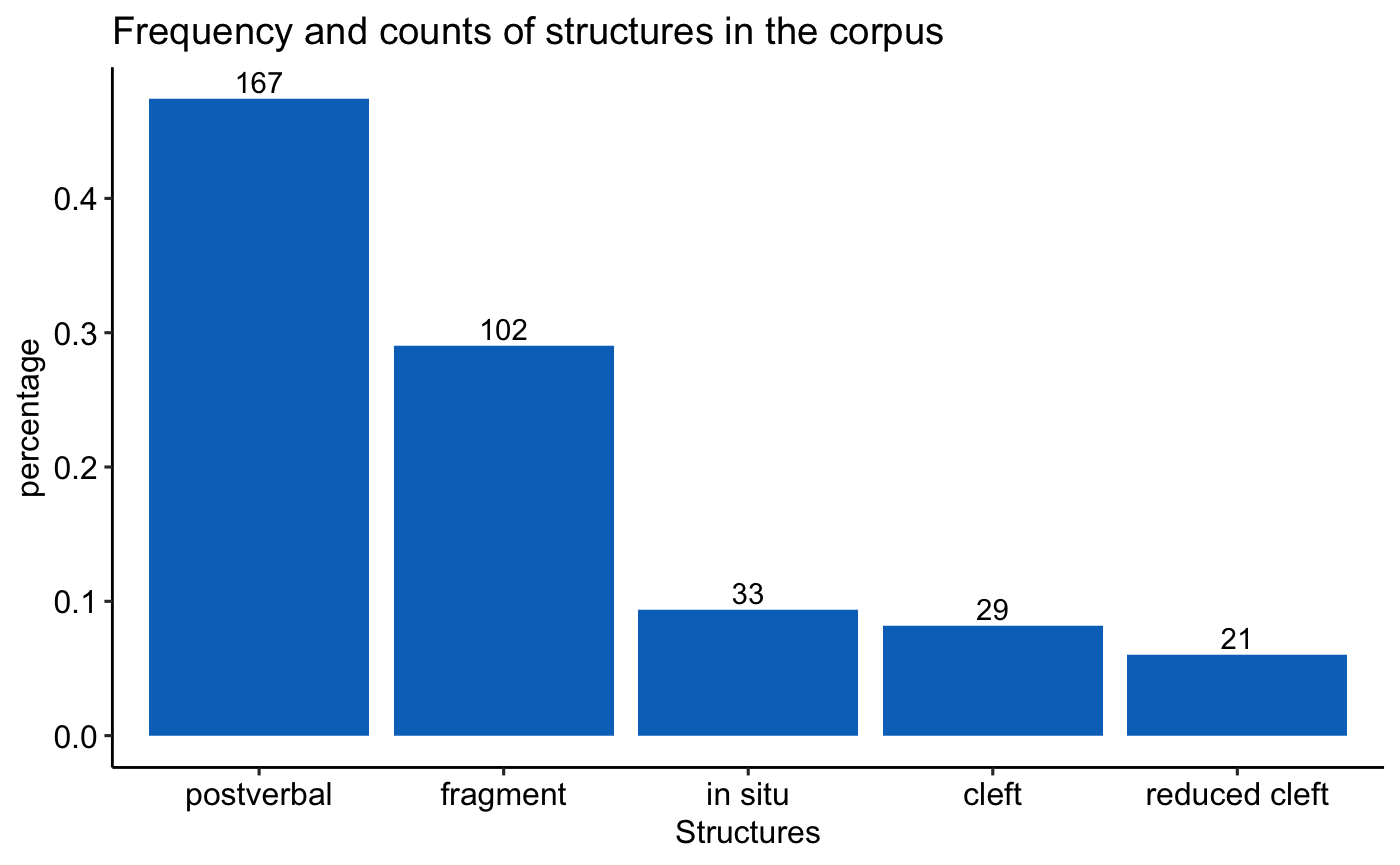
\includegraphics[width=0.7\textwidth]{Images/ES_structures_per.png}
    \caption{Frequency of answer types in Spanish}
    \label{fig:3:Plot1}
    % \label{fig:3:my_label}
\end{figure}

 As \figref{fig:3:Plot1} shows, Spanish speakers produced a total of 352 subject foci. Among the 352 critical items, 48\% (N=167) are postverbal subjects, 29\%  (N=102) are fragment answers, 9\% (N=33) are in situ subjects, 8\% (N=29) are clefts and 6\% (N=21) are reduced clefts. And so, according to this data set, the most frequent means to express focused subjects is the VS order. The corpus nonetheless shows variation in the type of answer. Speakers produced both full and elliptical structures with different distributions. 
 
 A Chi-square goodness-of-fit test was conducted to examine whether the distribution of structures differed from uniform. The result was highly significant, $\chi^2(4, N=352) = 365.15$, $p < 2.2 \times 10^{-16}$, indicating that some structures occurred much more frequently than others. Post-hoc pairwise comparisons (Bonferroni-corrected) showed that postverbal and fragment structures were significantly more frequent than in situ, cleft, and reduced cleft constructions (all $p < .001$). There were no significant differences among in situ, cleft, and reduced cleft structures (all $p = 1$). These results demonstrate that postverbal and fragment constructions dominate the distribution, while cleft and reduced cleft constructions are rare.
 
 The results for the overall frequency of the different focus types are presented in \tabref{tab:4.2}. The table shows the counts for the two focus types in the Spanish corpus, without breaking them into specific answering strategies.

\begin{table} 
\centering
\begin{tabular}{lr}
  \lsptoprule
Focus Type & Counts \\ 
  \midrule
 {Contrast} &  38 \\
 {Information} & 314 \\
   \lspbottomrule
\end{tabular}
\caption{Distribution of focus types}
\label{tab:4.2}
\end{table}



As can be seen from \tabref{tab:4.2}, among the 352 subject foci, 90\% (N=314) are information foci and only 10\% (N=38) contrastive foci. Overall, information focus appears to be the focus type most frequently produced. This result is in line with the literature on focus, according to which contrast is, by definition, a more marked IS-function than conveying new information \parencite{zimmermann2008contrastive, skopeteas2010focus}. 

\tabref{tab:4.3} reports the results for the relationship between different focus types and different answer types.

\begin{table}[ht]
\centering
\begin{tabular}{rrr}
  \lsptoprule
 & \textbf{Contrast} & \textbf{Information} \\ 
  \midrule
cleft &   3 &  26 \\ 
  fragment &  10 &  92 \\ 
  in situ &  10 &  23 \\ 
  postverbal &  12 & 155 \\ 
  reduced cleft &   3 &  18 \\ 
   \lspbottomrule
\end{tabular}
\caption{Distribution of focus types by focus structure.}
\label{tab:4.3}
\end{table}


 Among the 167 postverbal subjects, 155 (92\%) are information foci, while 8\% (N=12) are contrastive. Of the 102 fragments, 92 (91\%) are information and 9\% (N=10) are contrastive foci. Among the 33 in situ subjects, 23 (70\%) express new information and 10 (30\%) contrast. Among the 29 clefts, speakers conveyed 26 information foci (90\%) and only 3 (10\%) contrastive foci. Finally, among the 21 reduced clefts, 18 (86\%) are information foci and 3 (14\%) are contrastive.
 
 A Fisher's exact test was conducted to examine whether the proportion of contrastive versus informational focus differed across structures. The result was significant, $p = 0.001$, indicating that focus type depends on syntactic structure. Inspection of the data shows that in situ structures have the highest proportion of contrastive focus, whereas postverbal and fragment structures predominantly carry informational focus. Cleft and reduced cleft structures show small counts for contrastive focus, making the differences less reliable. These results suggest that in situ structures are particularly likely to convey contrastive focus.


\subsection{Discussion} \label{sub:4.5.1}
\subsubsection{Overview} \label{sub:4.5.1.1}
The corpus investigation revealed that the most frequent way to encode narrow focus on the subject in Spanish is by means of subject-verb inversion or postverbal subjects. This finding is in line with what the formal approaches to focus in Spanish have proposed so far (e.g., \cite{zubizarreta1998prosody}, \cite{gutierrez2013structural}, a.o., see \chapref{sec:2}). Diverging from these views, however, the data shows that postverbal subjects are by no means the only way to encode subject focus, and that the same function can be expressed by other strategies. For instance, speakers produced a considerable number of fragment answers and, albeit with a lower frequency, in situ subjects, clefts and reduced clefts, thus confirming that there is variation in the expression of focused subjects.

At the level of the type of focus, it is possible to observe that the information type was produced with greater frequency compared to the contrastive/corrective type. As mentioned above, this is also in line with previous literature that assumes a scale of markedness of pragmatic functions, where expressing contrast is considered to be a costlier operation than simply conveying non-presuppositional information \parencite{zimmermann2008contrastive, skopeteas2010focus}.

Based on these results, it is also possible to rule out the assumption of a one-to-one correlation between form and function (i.e., between focus type and syntactic structure), as all the strategies encode both focus types. A direct relationship between a specific type of focus and a single marking strategy is therefore excluded.
However, some variation can be observed in the frequency with which different strategies encode various focus types. For instance, while some structures (e.g., fragments or postverbal subjects) rarely encode contrast, others (e.g., in situ subjects) fulfill this function more frequently. This suggests that while no strategy is exclusively tied to a single focus type, certain constructions show a stronger preference for encoding particular focus functions.

\subsubsection{Postverbal subjects} \label{sub:4.5.1.2}

Postverbal subjects are the most frequent means used to express focused subjects in the Spanish data set. This is in line with formal accounts on focus that assume that among the subject NPs, it is possible to find all kinds of referring expressions: pronouns, proper names, definite and indefinite NPs and (negative) quantifiers. The focused subject can be found in sentence-final position ({\textit{Llegó} {[\textit{la policía}]}\textsubscript{\textsc{foc}} \normalsize `The police came')  or can be followed by another constituent ({\textit{Sí, bueno hemos llamado} {[\textit{los dos}}]\textsubscript{\textsc{foc}}} \normalsize \textit{a la policía} `Yes, well, we both called the police').

In \chapref{sec:5}, I report the result of a study where factors such as verb type, exhaustivity and givenness of the subject constituent are tested in relation with postverbal vs. preverbal subjects. I show that postverbal subjects correlate mostly with new subjects of unaccusative verbs, a result which is once again in line with previous literature on these structures (see, for instance, \cite{burzio1986italian}, on the association between unaccusatives and the VS order). 
Although all other answer types show a similar picture, postverbal subjects are the strategy that is most strongly associated with information focus (92\%), and exhibit the lowest rate of contrastive foci (8\%). It is interesting to note, though, that the same position can express different pragmatic inferences of focus; a finding that sharply contrasts with formal theories that assume two different syntactic positions for different focus types (see, for instance, the Cartographic Approach; \cite{rizzi1997fine}). 

Among the few cases of contrastive foci, it is possible to identify both occurrences of correction and, even if marginally, selection. Consider the two examples below:

 \ea \label{ex:3:16} \textbf{Correction:}\\
 (Speaking about the corpse)
\ea \textit{Pues, esta mañana lo han encontrado.}\\
 ‘Well, they found him this morning.'
\exi{a.} \textit{Bueno, lo ha encontrado} {[\textit{su mujer}]\textsubscript{\textsc{foc.}}}\normalsize\\
‘Well, his wife found him.' \hfill (\textit{sgs} Spanish, 7/8-9)   
\z \z 

 \ea \label{ex:3:17} \textbf{Selection:}
\ea \textit{¿Han bajado los dos?}\\
 ‘Did they both come downstairs?'
\ex \textit{Bueno, ha bajado} {[\textit{el marido}]\textsubscript{\textsc{foc}}} \normalsize \textit{porque la mujer estaba arriba}.\\
‘Well, the husband came down because the wife stayed upstairs.' \\
\hfill (\textit{sgs} Spanish, 17/45-46)   
\z \z 


In (\ref{ex:3:16}), the same speaker corrects himself/herself by using a postverbal subject, while in (\ref{ex:3:17}), speaker A gives a closed set of possible alternatives, and speaker B selects one of them. Thus, both contrast and information can be expressed by the same subject position. It remains to be assessed whether any difference can be observed in the prosodic contour of each function. However, such an analysis is outside the scope of this book.


\subsubsection{Fragments} \label{sub:4.5.1.3}

Spanish speakers produced a total of 102 fragment answers. It is worth noting that the second-most frequent strategy is an elliptical one (102/352); this is evidence of the fact that these answer types are far from uncommon in spontaneous speech.
The fragments produced in Spanish are almost exclusively full noun phrases. The corpus revealed a total of 99 NPs and only 3 personal pronouns among the 102.

 \ea \label{ex:3:18}
\ea \textit{Y, ¿Qué vecino encontró a la chica? }\\
 ‘And, which neighbour found the girl?'
\ex \textit{Pues,} {[\textit{su compañera de piso}]\textsubscript{\textsc{foc.}}}\normalsize\\
‘So, her flatmate.' \hfill (\textit{sgs} Spanish, 25/46-47)   
\z \z 


As for the type of focus expressed, in this case again, it is possible to observe an almost exclusive association with information focus (92/102), while contrast is expressed only marginally (10/102). This result is not surprising per se. An assertion containing a corrective focus has the communicative function of replacing the old value with a new one (see \cite{gussenhoven2008types}). To express such a function, speakers generally tend to express more rather than less material, and to resort to marked syntactic or prosodic configurations \parencite{zimmermann2008contrastive}. Thus, fragments are felicitous strategies when expressing new information, but rarely found in corrective/contrastive contexts. Additionally, the 10 cases of correction found in the Spanish data set almost never appear alone, but are generally accompanied by negative polarity items (e.g., \textit{No, la señora de arriba} `No, the lady from upstairs') or by discourse markers, such as \textit{bueno} `well'.


\subsubsection{In situ subjects} \label{sub:4.5.1.4}

The Spanish corpus also contains a limited number of focused preverbal subjects or focus in situ (N=33), where the subject appears either right at the beginning of the utterance or following DMs or negative polarity items. Unlike fragments, here it is possible to find a majority of NPs with a high referential level, such as personal pronouns or proper names; some definite NPs can also be found, while indefinites seem to be rather scarce (3 out of 33). 
Although there is once again a stronger association with information focus, it is possible to see that the association with contrast seems to be more frequent than in the other answer types. 
This finding is in line with previous research both at the level of contrast and at the level of information. On the one hand, in fact, theoretical approaches to focus (e.g., \cite{zubizarreta1998prosody}) argue that  focused in situ subjects are found solely when they express contrast rather than information\footnote{Even though the results reported here suggest that this claim should be expressed in terms of probabilistic frequencies rather than deterministic truths.}. On the other hand, \textcite{gabriel2007fokus} has argued in favor of the possibility of information focus to be expressed only prosodically, without involving movement of the constituents (see \chapref{sec:2}). As reported in \chapref{sec:2}, in Gabriel's experiment (\citeyear{gabriel2007fokus}), in situ focus is preferred with transitive verbs containing a fully realized object NP. The author provides an explanation in terms of cost of operations, arguing that it is easier for speakers to leave the subject in its in situ-position, and signal focus by a higher prosodic contour, rather than by moving the full object NP to a preverbal position, and producing a marked syntactic configuration. 

However, when the in situ subjects expressing contrastive focus (10/33) are excluded, only 6 out of 23 items fulfill this condition, i.e., only 6 sentences have a transitive verb with a fully-realized object NP (e.g., \textit{Sí,} [\textit{\textit{la familia}}]\textsubscript{\textsc{foc}} \normalsize \textit{denunció la desaparición} `Yes, the family signaled her disappearance'). The remaining tokens contain (di)transitive verbs with an object clitic (e.g., \textit{Sí,} [\textit{\textit{ella}}]\textsubscript{\textsc{foc}} \normalsize \textit{me ha avisado} `Yes, she warned me') or are accompanied by mono-argumental verbs (e.g., \textit{Pues,} [\textit{\textit{su mujer}}]\textsubscript{\textsc{foc}} \normalsize \textit{llegó.} `So, his wife arrived').

According to the literature, in situ subjects should bear prosodic prominence as the iconic means of signaling to the hearer that that particular constituent is the value satisfying his/her request for information, while the rest of the sentence is de-accented (e.g., \cite{fery2001focus}). As mentioned above, a prosodic analysis of these items is outside the scope of this book. However, in situ subjects will be analyzed quantitatively in \chapref{sec:5}, where I investigate the semantic and pragmatic factors that trigger these structures, and compare them to postverbal subjects.

\subsubsection{Clefts} \label{sub:4.5.1.5}

A reduced number of focused subjects is also expressed by clefts (N=29). Among the cleft types in the corpus, it is possible to find some formats introduced by the copula \textit{ser} `to be' (e.g., \textit{Pues, fueron} [\textit{los padres}]\textsubscript{\textsc{foc}} \normalsize \textit{que la vieron por última vez} `So, it was the parents that saw her for the last time'), the verb \textit{haber} `to have' (e.g., \textit{Sì, de hecho hay} [\textit{un par de hombres}]\textsubscript{\textsc{foc}} \normalsize \textit{que vienen siempre} `Yes, actually, there are a couple of men that always pass by'), or a wh-element (e.g., \textit{Quien la visita son} [\textit{sus nietos}]\textsubscript{\textsc{foc}} \normalsize `Who visits her are his grandchildren'), and followed (or preceded) by a relative clause.
Among the focused subjects contained in the clefted element it is possible to find a majority of definite NPs (N=27), only 1 pronoun and 1 indefinite. Interestingly, the corpus  also contains a limited number of inverted pseudo-clefts (terminology adopted by \cite{feldhausen2015oraciones}), where the clefted element precedes the copula (e.g., [\textit{Ella}]\textsubscript{\textsc{foc}} \normalsize \textit{ha sido la que se ha encontrado el cuerpo} `It was her who found the body').

As mentioned in \chapref{sec:2}, while the clefted constituent is generally considered to be the contrastively focused element in Spanish (see, e.g., \cite{zubizarreta1999word, van2005exploring}), \textcite{cabrera1999funciones} and \textcite{feldhausen2015oraciones} state that simple clefts on the one hand and (inverted) pseudo-clefts on the other hand have different information-structural properties. The results of the Spanish dataset seem to corroborate this finding, showing that 26 out of 29 clefts express information focus, while only 3 express contrast. This supports the claim that contrast/correction is only one of the possible information-structural functions associated with Spanish clefts, and that these structures can also be used to convey new information, albeit with a limited frequency.
 
\subsubsection{Reduced clefts} \label{sub:4.5.1.6}

Reduced clefts are the least frequent means of marking focus in the Spanish corpus (N=21). They are introduced mainly by a copula (e.g., \textit{Pues, ha sido} [\textit{su compañera de piso}]\textsubscript{\textsc{foc}} \normalsize `So, it was her flatmate'), although some can be found with the verb `to have' (e.g., \textit{Pues, habían, como yo calculo, que} [\textit{unas 8 personas}]\textsubscript{\textsc{foc}} \normalsize \textit{o por ahí} `So, there were some 8 people or something like that'). The sentences could be either main clauses or embedded ones (e.g., \textit{Sabemos que fue} [\textit{el lampista}]\textsubscript{\textsc{foc}} \normalsize `We know that it was the plumber'). It is possible to find any kind of NPs associated with reduced clefts, although the most common collocations are definite NPs with \textit{ser} and indefinites with \textit{haber}. As for the association of these structures with focus type, reduced clefts almost exclusively appear with information focus, with only 3 tokens expressing contrast. Overall, it seems that contrast is only marginally expressed by all structures, especially elliptical ones.

\section{Corpus results for French} \label{sub:4.6}

In this section, I report the results for the French-focused subjects found in the corpus. As was the case for the Spanish corpus, I first present all the answer types that encode narrow focus on the subject, without differentiating among different focus types. I then show the results for the overall distribution of the two focus types, and I finally look at the interaction between different answer types and different focus types. 
\begin{figure}
\centering
    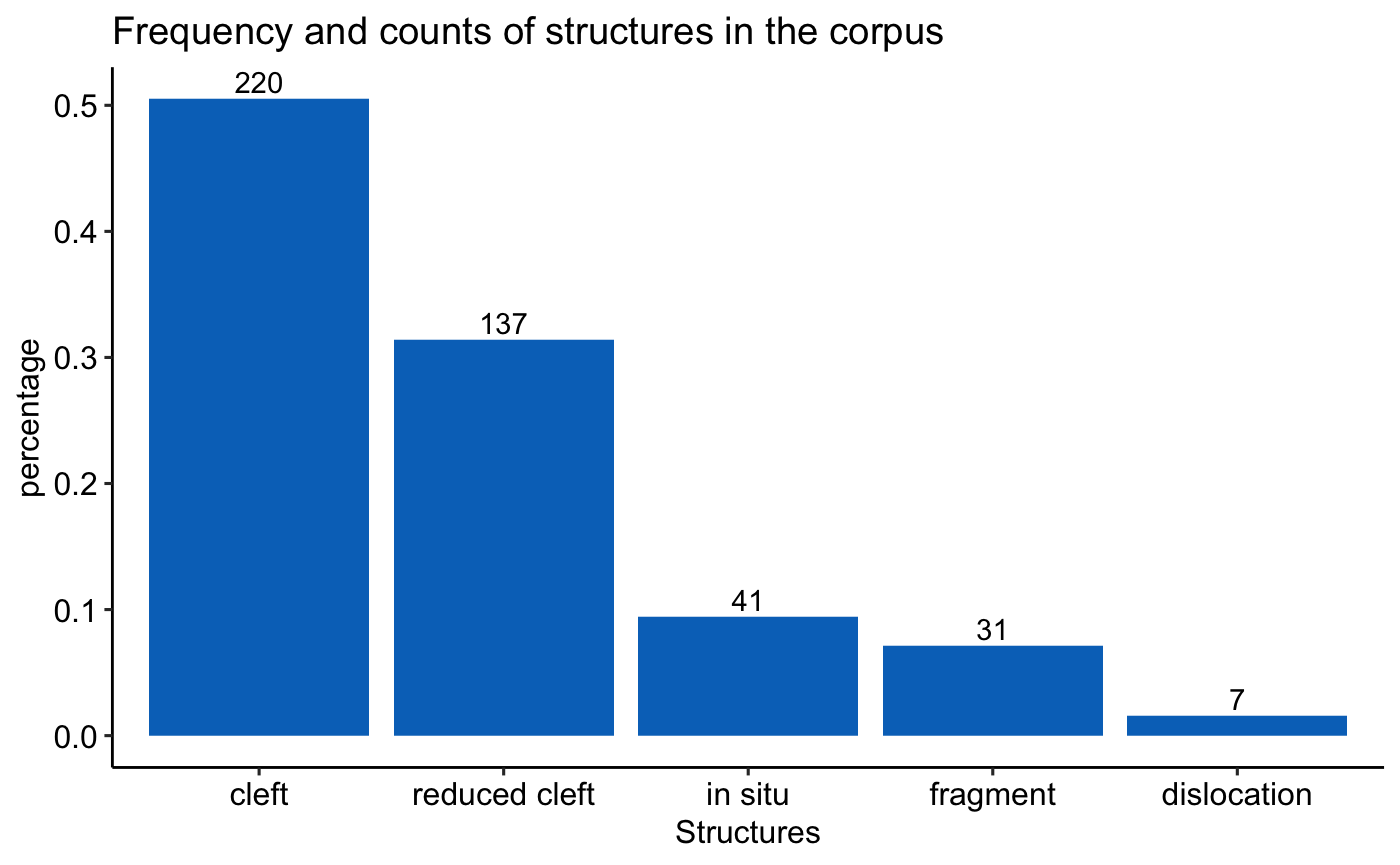
\includegraphics[width=0.7\textwidth]{Images/FR_structures_per.png}
    \caption{Frequency of answer types for French}
    \label{fig:3:Plot2}
    % \label{fig:3:my_label}
\end{figure}


\figref{fig:3:Plot2} shows that French speakers produced a total of 436 subject foci. Among the 436 sentences, 50\% (N=220) are clefts,\footnote{Note that I do not differentiate at this stage among different cleft formats. This implies that the label \textsc{cleft} includes cases of \textit{c'est}-, \textit{il y a}- and pseudo-clefts.} 31\% (N=137) are reduced clefts, 9\% (N=41) are in situ subjects, 7\% (N=31) are fragment answers and only 3\% (N=7) are dislocations.

A Chi-square goodness-of-fit test was conducted to examine whether the distribution of structures differed from uniform. The result was highly significant, $\chi^2(4, N = 436) = 365.4$, $p < 2.2 \times 10^{-16}$, indicating that some structures occurred much more frequently than others.%{check this formula}
Post-hoc pairwise comparisons (Bonferroni-corrected) revealed that clefts occurred significantly more often than reduced clefts, in situ constructions, fragments, and dislocations (all $p < .001$). All other pairwise comparisons were significant ($p \leq .001$), indicating that most structures differed in frequency from each other.

\tabref{tab:4.4} shows that French speakers produced 85\% (N=370) information foci and 15\% (N=66) contrastive foci. This result is somewhat similar to the results of the Spanish data, reported in \tabref{tab:4.2}, where information focus is by far the most frequent type. \tabref{tab:4.5} shows the proportion of different focus types for each answering strategy.

\begin{table}[ht]
\centering
\begin{tabular}{rr}
  \lsptoprule
Focus Type & Count \\ 
  \midrule
 {Contrast} &  66 \\
 {Information} & 370 \\
   \lspbottomrule
\end{tabular}
\caption{Distribution of focus types}
\label{tab:4.4}
\end{table}

\begin{table}[ht]
\centering
\begin{tabular}{rrr}
  \lsptoprule
 & contrast & information \\ 
  \midrule
cleft &  46 (22\%) & 174 (78\%) \\ 
  reduced cleft &   7 (3\%) & 130 (97\%)\\ 
  in situ &  10 (24\%) &  31 (76\%) \\ 
  fragment &   1 (3\%) &  30 (97\%)\\ 
  dislocation &   2 (29\%) &   5 (71\%) \\ 
   \lspbottomrule
\end{tabular}
\caption{Distribution of focus types by focus structure}
\label{tab:4.5}
\end{table}

Post-hoc pairwise comparisons (Bonferroni-corrected) were conducted to examine which structures differed in their distribution of focus types. The results showed that clefts differed significantly from all other structures (reduced clefts, in situ constructions, fragments, dislocations; $p < .001$), and reduced clefts differed significantly from clefts, fragments, and dislocations ($p < .001$). in situ constructions and fragments did not differ significantly from each other ($p = 1.00$), indicating similar distributions of contrastive and informational focus. All other pairwise comparisons were significant ($p \leq .01$), demonstrating that the choice of structure certainly affects the type of focus realized.


\subsection{Discussion} \label{sub:4.6.1}
\subsubsection{Clefts} \label{sub:4.6.1.1}

Half of the answer types produced by speakers (N=220) were subject cleft sentences. As mentioned above, the cleft category reported in \figref{fig:3:Plot2} does not differentiate among different cleft types. A closer look reveals that the corpus contains 109 \textit{c'est}-clefts (e.g., \textit{C'est} [\textit{sa femme}]\textsubscript{\textsc{foc}} \normalsize \textit{qui l'a trouvé} `It's his wife who found him'), 98 \textit{il y a}-clefts (e.g., \textit{Il y a} [\textit{\textit{une autre étudiante}}]\textsubscript{\textsc{foc}} \normalsize \textit{qui vit dans l'immeuble} `There is another student that lives in the building') and 13 pseudo-clefts (e.g., \textit{Ce qui m'intéresse bien c'est} [\textit{s\textit{on mari}}]\textsubscript{\textsc{foc}} \normalsize `What interests me the most is her husband').

Thus, not only \textit{c'est}-, but also other cleft formats can encode subject focus in French; this is a finding that contradicts claims found mainly in the theoretical tradition (e.g., \cite{lambrecht1996information}).
The fact that a considerable number of \textit{il y a}-clefts, for instance, express narrow focus on the subject seems to confirm Karssenberg's (\citeyear{karssenberg2017oiseaux}) corpus study, in which the author shows that \textit{il y a}-clefts do not necessarily exhibit an all-new focus type. 
Here again, there is a strong association with information focus, with a limited number of clefts expressing contrast. \textcite{lambrecht1996information} claims that pragmatic inferences like contrast can only be expressed by \textit{c'est}-clefts. A closer look at the different cleft types reveals that a small number of \textit{il y a}-clefts is also associated with contrast (N=9). However, none of them expresses correction stricto sensu, but rather selection from a set of closed alternatives (as in (\ref{ex:3:19})). In contrast, all cases of correction are indeed expressed by \textit{c'est}-clefts.

 \ea \label{ex:3:19}
\ea	\textit{Et, au niveau de cet étage, les locataires sont là?}\\
 ‘And, speaking about this floor, are the tenants there?'
 \exi{a.} \textit{Ou ils sont en vacances?}\\
 ‘Or are they on holidays?'
\ex \textit{Il y en a} {[\textit{deux}]\textsubscript{\textsc{foc}}} \normalsize \textit{en vacances et} {[\textit{un}]\textsubscript{\textsc{foc}}}  \textit{qui est encore là}.  \\
‘So, there are two on holidays and the one that is still there.' \\
\hfill (\textit{sgs} French, 7/182-184)    
\z \z 


It must be noted that the answer contained in (\ref{ex:3:19}b) is ambiguous between a contrastive focus and a contrastive topic reading. The difference between contrastive focus and contrastive topic is subtle but central in the study of information structure.

Contrastive focus identifies an element that contrasts with other possible alternatives in the discourse. It answers a wh-question or corrects a presupposition. A constituent marked as contrastive topic, on the other hand, introduces a topic–comment partition where the topic is contrasted with alternative topics (e.g., A: What about Paul and Marie? What did they buy? B: Well, [PAUL]\tiny{CT} \normalsize bought the wine, and [MARIE]\tiny{CT} \normalsize bought the cheese). It signals that the speaker will provide partial answers across alternatives, often leaving the door open to further elaboration \parencite{krifka2008basic}.

The example in (\ref{ex:3:19}) is ambiguous because the speaker does not explicitly formulate a wh-question about the subject, such as \textit{Who is currently in the building?}. Consequently, the yes/no question in (\ref{ex:3:19}a) could be interpreted either as \textit{Which neighbour is in the building?} (i.e., contrastive focus) or as \textit{What are the neighbours doing?} (i.e., contrastive topic). Given the contextual setting of the interview, in which participants are asked to solve a murder case, I assume that the communicative intention of the speaker was to determine which neighbour is present on each floor in order to narrow down the pool of potential culprits. For this reason, I analyze the sentence in (\ref{ex:3:19}b) as an instance of contrastive focus.
 
Concerning the NP types associated with each cleft type, there is a strong tendency towards the following collocations: pronouns and definite NPs with \textit{c'est}-clefts, indefinite NPs with \textit{il y a}-clefts and heavy NPs with pseudo-clefts. The question of the interaction between cleft type and other factors, such as NP type or verb type will be discussed in detail in \chapref{sec:5}.

\subsubsection{Reduced clefts} \label{sub:4.6.1.2}

French speakers also produced a considerable number of reduced clefts (N=137). As was the case for the Spanish data set, it is interesting to note that the second most frequent strategy is an elliptical one; this is further evidence in support of the claim that these structures are far from being uncommon in spontaneous speech.

The corpus shows two types of reduced clefts: 77 reduced \textit{c'est}- (e.g., \textit{C'est} [{\textit{moi}}]\textsubscript{\textsc{foc}} \normalsize `It's me') and 60 of the \textit{il y a}-type (e.g., \textit{Il y a} [{\textit{un homme}}]\textsubscript{\textsc{foc}} \normalsize \textit{aussi} `There is also a man'). Interestingly, a closer look at the association between the two types of reduced clefts and the NP type contained in the clefted element reveals a similar pattern to the one found for full clefts: a majority of pronouns, proper names and definite NPs occur with the \textit{c'est-}type, while a majority of indefinite NPs collocate with \textit{il y a}-reduced clefts.

In a way similar to the other strategies, reduced clefts express contrast in only a very limited number of cases, and have an almost total association with information focus. 

It is interesting to note that some items annotated as reduced clefts in French contain the start of a relative clause that is, however, incomplete (i.e., ``Trailing off'', e.g., \textit{Non, ça doit être}  [{\textit{les flics}}]\textsubscript{\textsc{foc}} \normalsize \textit{qui ont...}`No, it must be the cops that have...'). These cases might be taken as evidence for the reduction hypothesis \parencite{jenkins2017cleft} if one assumes that the speaker had the intention of producing a full cleft but, for discourse-related reasons, left the sentence incomplete. Nevertheless, this phenomenon does not occur regularly, and the number of cases is not large enough to provide this kind of generalizations.

\subsubsection{\textbf{In situ}} \label{sub:4.6.1.3}

Some in situ strategies have also been used to express subject focus (N=41). It is remarkable to observe that the majority of in situ focused subjects are quantifiers such as \textit{tout le monde} `everybody' or negative quantifiers, such as \textit{personne} `nobody'. Some personal pronouns, proper names and definite NPs are also present, while not a single case of indefinite NP has been found. 

The presence of in situ foci in this dataset goes against the claim that French completely bans foci from the preverbal position \parencite[492]{lambrecht2001framework} because of its prosodic peculiarities (phrase-final stress instead of word stress). Rather, it is in line with \textcite{fery2001focus}, who found robust experimental evidence in favor of the existence of preverbal foci in French. The corpus shows that these strategies are not very frequent, but they can express both information focus
and, to a lesser extent, contrastive focus. A closer look at the contrastive cases reveals that the in situ strategy can be used to express both selection (as in (\ref{ex:3:20})) and correction (as in (\ref{ex:3:21})):

 \ea \label{ex:3:20}
\ea \textit{Donc dispute violente?}\\
 ‘So, was it a violent fight?'
 \ex \textit{Ouais, carrément.}\\
 ‘Yes, totally.'
 \exi{a.} \textit{Qui insultait qui?}\\
 ‘Who was insulting whom?'
\exi{b.} {[\textit{Elle}]\textsubscript{\textsc{foc}}} \normalsize \textit{insultait} {[\textit{lui}]\textsubscript{\textsc{foc.}}}\footnote{It has to be pointed out that this is an interesting case of double focus: apart from focus on the subject, the same utterance also contains focus on the object. In this case, the SVO order could be an artifact of this phenomenon. However, other occurrences of in situ subjects can be found in association with selection.}\\
‘She insulted him.' \hfill (\textit{sgs} French, 93/190-193)   
\z \z 

 \ea \label{ex:3:21}
\ea \textit{On l'a retrouvé où?}\\
 ‘Where was he found?'
 \ex \textit{On l'a retrouvé chez elle.}\\
 ‘He was found at her place.'
 \exi{a.} \textit{m.}\\
 ‘m.'
\exi{b.} {[\textit{Je}]\textsubscript{\textsc{foc}}} \normalsize \textit{l'ai retrouvé}. \\
‘I found him.' \hfill (\textit{sgs} French, 63/93-96)    
\z \z 


As is the case with the Spanish in situ subjects, a prosodic analysis would reveal further insights into these strategies, especially in the case of correction, where a higher pitch tone is expected on the new variable. I leave such an analysis for further research.


\subsubsection{Fragments} \label{sub:4.6.1.4}

Unlike the Spanish speakers, the French speakers only produced 27 fragment answers. It is interesting to note that some answering strategies that are numerous in the Spanish corpus are very rare in the French one. This difference will be discussed in the comparative analysis in \sectref{sub:4.7}.

The majority of the fragments found in this dataset express information focus, while only 1 out of 27 is, in fact, associated with contrast. At the level of the NP, the majority of subjects are definite noun phrases; the remainder consists of a few pronouns and only 2 indefinite NPs.

\subsubsection{Dislocations}

As mentioned above, dislocations can be found in the French but not in the Spanish corpus. They are, however, extremely scarce (N=7). The  dislocated constituents are mostly strong personal pronouns (especially the first person singular \textit{moi} I') or definite NPs. Although dislocations are generally treated as topic-marking strategies, the corpus shows that some speakers have made use of these constructions to mark focus. The fact that subject focus can be marked by a dislocation is in line with the prosodic requirements of French and with Féry's (\citeyear{fery2001focus}) Phrasing Hypothesis: by positioning the subject constituent in the left periphery, the speaker creates two intonational phrases, one for the focused subject and one for the background proposition. The subject can thus receive prosodic prominence by virtue of being positioned phrase-finally, and can be marked as focus. Even if extremely scarce, it is possible to see that dislocated subjects can express both information and contrastive focus.

\section{Comparative analysis of frequencies: the ``copy” hypothesis} \label{sub:4.7}
Looking at the overall distribution, the first important consideration is that focused subjects appear to be relatively infrequent in both languages. This finding is in line with what \textcite{lambrecht1996information} or \textcite{skopeteas2010focus} have claimed about the degree of markedness of the subject in focus (see \chapref{sec:1}), i.e., the assumption of a default association ‘subject = topic’, implying that deviations from this configuration should be structurally marked (see \cite[490]{lambrecht2001framework}; \cite[336]{zerbian2007investigating}; \cite{hartmann2007place}). This markedness seems to be reflected not only in the association between subject focus and non-canonical forms but also in the frequency of the focus-marking strategies produced. It is interesting to note, though, that the data shows variation at the level of the strategies that express the same pragmatic function. In both languages, speakers produced the same number of answering strategies (5 for each language), albeit with different frequencies. The fact that a focused subject can be expressed by other means such as elliptical forms is not surprising per se. However, to the best of my knowledge, there have been no studies  conducted so far that investigate the frequency with which different strategies are used language-internally, or that compare French and Spanish in this respect.

Overall, the results from the two sub-corpora appear to support the theoretical claim that, due to its rhythmic structure, French exhibits a relatively rigid word order and relies on constructional strategies to convey certain information-struc\-tur\-al functions. In contrast, Spanish achieves this more economically through word order alternation. While the findings reported here reinforce this claim, the variation observed in both languages suggests that these are tendencies rather than rigid rules. In other words, although Spanish postverbal subjects and French clefts are the most common strategies, they are by no means the only ones.

The absence of postverbal subjects in the French data supports Lahousse's (\citeyear{lahousse2006, Lahousse2011}) claim that postverbal subjects in French are now limited to a narrow range of linguistic contexts and lack the same information-structural properties as their Spanish counterparts. On the other hand, clefts appear in both languages, as the results suggest, though their distribution varies significantly. The observation that clefts in the Spanish corpus represent only 8\% of the total answers (compared to 50\% in the French corpus) suggests that, \textit{ceteris paribus}, Spanish speakers tend to favor more economical strategies, such as subject-verb inversion, over the more complex and construction-heavy cleft sentences.

The in situ strategy, on the other hand, appears to be a disfavored option in both languages. Notably, both Spanish and French in situ focused subjects almost never appear as indefinite NPs. This finding seems to confirm a tendency observable in many languages: positioning a brand-new referent in the sentence-initial slot is generally avoided. It is well known that not all NP types are equally felicitous in the sentence-initial position, and this slot appears to be influenced by the ``definiteness effect” (see e.g., \cite{keenan1976foregrounding}; \cite{mcnally1998existential}), which suggests that highly accessible referents are preferred over less accessible ones. Moreover, as mentioned earlier, French employs syntactic strategies, such as \textit{il y a}-clefts, to avoid placing ``bad” subjects at the beginning of the sentence \parencite{Karssenberg+2018}. Given that no instances of indefinite NPs are associated with the Spanish in situ strategy, it can be argued that this tendency also applies to Spanish.
Thus, the results are innovative in several respects. First, they demonstrate that there is no deterministic relationship between form and function, indicating that speakers utilize various means to express the same pragmatic function. Second, they provide frequencies for elliptical strategies, illustrating that similar structures can be found in both languages.

The findings regarding elliptical answers are particularly interesting if observed from a comparative perspective: although both French and Spanish have the possibility to express the same function through either a reduced cleft or a fragment, the distribution of these strategies shows an opposite tendency in the two languages. For Spanish, fragments appear with a frequency that is comparable to reduced clefts in French (and not to their French counterpart), while reduced clefts in Spanish are as infrequent as fragments in French.
How can we account for this puzzling finding? In other words, why do French speakers prefer to use a reduced cleft when they could opt for a more economical strategy like a fragment?

One possible explanation may be related to the typological differences between the two languages. Spanish is typologically a pro-drop language, whereas French is not. Consequently, even when producing elliptical answers, French speakers may prefer a strategy in which the subject position is overtly filled by an element, such as the non-referential pronoun \textit{c'} that accompanies the copula in a reduced cleft construction. If this explanation is plausible, we would expect to observe similar tendencies when comparing other null subject vs. non-null subject languages, for instance Italian and Brazilian Portuguese. In these languages, focused subjects are reportedly expressed by postverbal subjects and clefts, respectively \parencite{kato2006focus}.

Similarly, the preference for reduced clefts in French could be linked to the rhythmic structure of this language (phrase-final stress). Since French supposedly does not assign prosodic prominence on a word alone, the presence of the pronoun \textit{c'} or \textit{il} and the corresponding copulas or verb \textit{avoir} allows speakers to create phrasing, and, as is the case for full clefts, to respect the prosodic requirements of the language.

Another possible explanation could be related to the Reduction Hypothesis \parencite{jenkins2017cleft}: assuming that both reduced clefts and fragments are indeed syntactically elliptical sentences, derived from their full counterparts, we could postulate that, when speakers intend to produce a subject in focus with an elliptical form, they have a stronger tendency to ``copy” the structure of the strategy they use more frequently (e.g., a cleft in French), and simply omit the background part for discourse-related reasons. This would explain why reduced clefts are more frequent in French, where the most common way to express a focused subject is a cleft, and why fragments are more frequent in Spanish, where the default way of expressing the same function is through a postverbal subject.

If this explanation holds true, we would expect to observe a high frequency of reduced clefts in French for the realization of subject focus, but not, for instance, for object focus. It is well established that French primarily employs clefts as a focusing strategy for subjects, while for focusing direct objects, speakers tend to use more economical means, such as in situ strategies (SV[O]\textsubscript{\textsc{foc}} \normalsize) \parencite{skopeteas2010focus, SkopeteasFanselow2011, destruel2016focus}. Therefore, if a similar study were conducted focusing on objects rather than subjects, one would expect to find a higher number of fragment answers as the corresponding elliptical strategy for object focus. Since the present study focuses exclusively on subject focus, these questions are left for future research.

The three explanations suggested above are not contradictory; rather, they are interconnected. Due to the typological and prosodic characteristics of the language, French tends to favor cleft sentences, while Spanish relies on subject-verb inversion as the preferred means of focusing the subject. However, as mentioned earlier, these claims should be interpreted as probabilistic rather than deterministic predictions. When speakers choose to produce an elliptical form, they retain the focused element from the corresponding full form while omitting the presupposed part of that structure.
The alternation between complete and elliptical forms will be further explored in the next chapter, where I examine the contexts that trigger the use of full versus elliptical strategies in both languages, analyzing the answer types in relation to the type of QUD they address.
 

\section{Summary} \label{sub:4.8}
The corpus study reported in this chapter has investigated the frequency of different strategies to mark focus on the subject in Spanish and French. The findings for both sub-corpora have shown that there are different ways of expressing the same IS-function, and that speakers produced both full and elliptical answers.
Moreover, the chapter has investigated possible associations between different strategies and different focus types. While the type of focus most frequently found in both languages are new information focus, some cases of contrast are also visible.

Interestingly, almost all the strategies can be found in the two languages (with the exception of postverbal subjects for French and dislocations for Spanish). The frequencies in each language, however, differ considerably.
Reduced clefts, for instance, are the second-most common means in French but the most infrequent in Spanish. Moreover, the most frequent elliptical strategy in Spanish appears to be fragment answers, a structure that was very rare in the French corpus. To explain this difference in frequency, I have proposed the ``copy” hypothesis, which suggests that speakers tend to replicate the focused part of the corresponding full structure most common in their language, while omitting the background information. The question of why speakers choose to omit the background proposition and express only the focused element will be addressed in the next chapter.
